\documentclass[10pt,a4paper]{article}

\usepackage[margin=0.7in,top=0.75in,bottom=0.7in]{geometry}
\usepackage[T1]{fontenc}
\usepackage{lmodern}
\usepackage{microtype}
\usepackage{xcolor}
\usepackage{hyperref}
\usepackage{listings}
\usepackage{booktabs}
\usepackage{tikz}
\usetikzlibrary{positioning,arrows.meta,shapes.geometric,shapes.symbols,fit,backgrounds,calc,decorations.pathreplacing}
\usepackage{enumitem}
\usepackage{titlesec}
\usepackage{fancyhdr}
\usepackage{array}
\usepackage{multicol}

% Colors
\definecolor{cmpblue}{HTML}{0B5FFF}
\definecolor{cmpdark}{HTML}{0B1F3A}
\definecolor{cmpgreen}{HTML}{0E8F4E}
\definecolor{cmpred}{HTML}{C0392B}
\definecolor{cmporange}{HTML}{E67E22}
\definecolor{codebg}{HTML}{F6F8FA}
\definecolor{codekey}{HTML}{0B5FFF}
\definecolor{codestr}{HTML}{0E8F4E}
\definecolor{codecmt}{HTML}{6A737D}
\definecolor{boxbg}{HTML}{EEF4FF}
\definecolor{okbg}{HTML}{E8F7EE}

\hypersetup{
    colorlinks=true,
    linkcolor=cmpblue,
    urlcolor=cmpblue,
    citecolor=cmpblue,
    pdftitle={Compresr SDK -- Integration Guide},
    pdfauthor={Compresr}
}

\titleformat{\section}{\large\bfseries\color{cmpdark}}{\thesection}{0.55em}{}
\titleformat{\subsection}{\normalsize\bfseries\color{cmpdark}}{\thesubsection}{0.45em}{}
\titlespacing*{\section}{0pt}{8pt}{4pt}
\titlespacing*{\subsection}{0pt}{6pt}{3pt}

\pagestyle{fancy}
\fancyhf{}
\fancyhead[L]{\footnotesize\color{cmpdark}Compresr SDK --- Integration Guide}
\fancyhead[R]{\footnotesize\color{cmpdark}\thepage}
\renewcommand{\headrulewidth}{0.4pt}

\lstdefinelanguage{pythonx}{
    language=Python,
    morekeywords={async,await,match,case,self,cls},
}
\lstset{
    language=pythonx,
    backgroundcolor=\color{codebg},
    basicstyle=\ttfamily\scriptsize,
    keywordstyle=\color{codekey}\bfseries,
    stringstyle=\color{codestr},
    commentstyle=\color{codecmt}\itshape,
    showstringspaces=false,
    breaklines=true,
    breakatwhitespace=true,
    columns=fullflexible,
    keepspaces=true,
    frame=single,
    rulecolor=\color{codebg!60!black!20},
    framerule=0.4pt,
    framesep=3pt,
    xleftmargin=6pt,
    xrightmargin=4pt,
    aboveskip=4pt,
    belowskip=4pt,
    literate={->}{{$\rightarrow$}}1 {<-}{{$\leftarrow$}}1
}

\setlist{itemsep=1pt,topsep=2pt,parsep=0pt}

\title{\vspace{-3em}\Large\bfseries\color{cmpdark}Compresr SDK --- LangChain/LangGraph Integration \& the Web Search Tool}
\author{}
\date{}

\begin{document}
\maketitle
\vspace{-3em}

% =====================================================================
\section{Architecture}
% =====================================================================

\noindent The whole SDK is one substitution: replace your provider client with \texttt{CompressionClient} and the same call-site code (\texttt{client.messages.create(...)}) keeps working --- except every tool result now passes through Compresr middleware before reaching the LLM.

\begin{center}
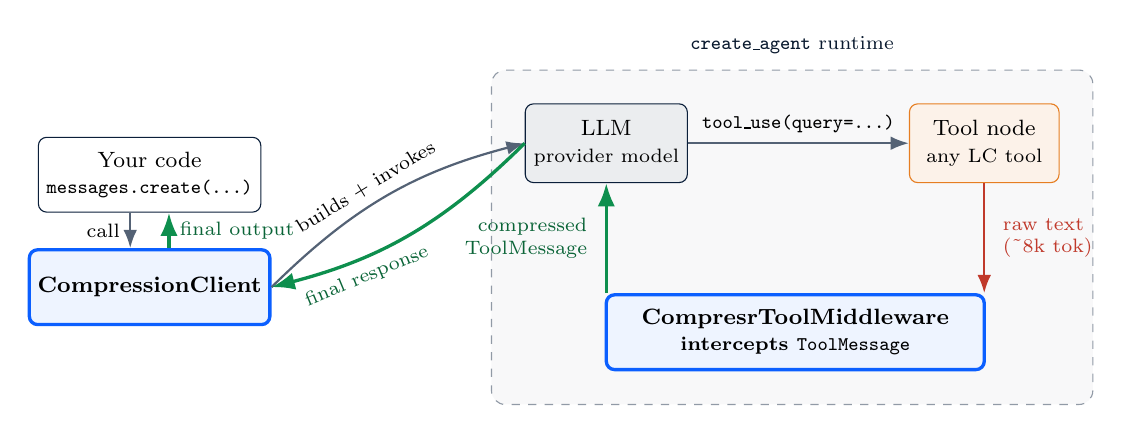
\begin{tikzpicture}[
  font=\footnotesize,
  entry/.style={draw=cmpdark,rounded corners=3pt,fill=white,
                minimum height=0.95cm,minimum width=2.8cm,align=center,inner sep=3pt},
  cliBox/.style={draw=cmpblue,very thick,fill=boxbg,rounded corners=3pt,
                 minimum height=0.95cm,minimum width=2.8cm,align=center,inner sep=3pt,
                 font=\footnotesize\bfseries},
  llm/.style={draw=cmpdark,rounded corners=3pt,fill=cmpdark!8,
              minimum height=1.0cm,minimum width=1.9cm,align=center,inner sep=3pt},
  tool/.style={draw=cmporange,rounded corners=3pt,fill=cmporange!10,
              minimum height=1.0cm,minimum width=1.9cm,align=center,inner sep=3pt},
  mwBox/.style={draw=cmpblue,very thick,fill=boxbg,rounded corners=3pt,
                minimum height=0.95cm,minimum width=4.8cm,align=center,inner sep=3pt,
                font=\footnotesize\bfseries},
  arr/.style={-{Latex},draw=cmpdark!70,thick},
  arrhot/.style={-{Latex},draw=cmpred,thick},
  arrok/.style={-{Latex},draw=cmpgreen,very thick},
]
% LEFT: entry stack (vertical)
\node[entry] (you) at (0,0) {Your code\\\scriptsize\texttt{messages.create(...)}};
\node[cliBox,below=0.45cm of you] (cli) {CompressionClient};

% RIGHT: agent runtime -- rectangular loop layout (WIDER)
\node[llm] (llm) at (5.8,0.4) {LLM\\\scriptsize provider model};
\node[tool] (tool) at (10.6,0.4) {Tool node\\\scriptsize any LC tool};
\node[mwBox] (mw) at (8.2,-2.0) {CompresrToolMiddleware\\\scriptsize intercepts \texttt{ToolMessage}};

% Frame for runtime
\begin{scope}[on background layer]
  \node[draw=cmpdark!45,dashed,rounded corners=5pt,fill=cmpdark!3,
        fit=(llm)(tool)(mw),inner sep=12pt] (frame) {};
\end{scope}
\node[font=\scriptsize\color{cmpdark!80!black},anchor=south,yshift=2pt] at (frame.north) {\texttt{create\_agent} runtime};

% Entry vertical -- request down, output up (two parallel arrows)
\draw[arr]   ([xshift=-7pt]you.south) -- node[left,font=\scriptsize]{call} ([xshift=-7pt]cli.north);
\draw[arrok] ([xshift=7pt]cli.north) -- node[right,font=\scriptsize\color{cmpgreen!70!black}]{final output} ([xshift=7pt]you.south);

% Client <-> LLM provider (request out, response back) -- bowtie of arcs.
% Labels shifted toward the client end so they don't collide with the
% "compressed ToolMessage" label sitting just south-west of the LLM.
\draw[arr]   (cli.east) to[bend left=15]  node[above,sloped,font=\scriptsize,pos=0.45]{builds + invokes} (llm.west);
\draw[arrok] (llm.west) to[bend left=15]  node[below,sloped,font=\scriptsize\color{cmpgreen!70!black},pos=0.7]{final response} (cli.east);

% Rectangular loop inside runtime:
% top: LLM -> Tool
\draw[arr] (llm.east) -- node[above,font=\scriptsize]{\texttt{tool\_use(query=...)}} (tool.west);
% right side: Tool down to MW (vertical)
\draw[arrhot] (tool.south) -- node[right,font=\scriptsize\color{cmpred},xshift=3pt,align=left]
                              {raw text\\(\textasciitilde 8k tok)}
                              (tool.south |- mw.north);
% left side: MW up to LLM (vertical)
\draw[arrok] (llm.south |- mw.north) -- node[left,font=\scriptsize\color{cmpgreen!70!black},xshift=-3pt,align=right]
                                         {compressed\\ToolMessage}
                                         (llm.south);
\end{tikzpicture}
\end{center}

% =====================================================================
\section{Part 1 --- Wrapping any LangChain / LangGraph tool}
% =====================================================================

If you have a LangChain tool, you already have a Compresr-compressible tool. No subclassing, no decoration. Three integration paths:

\subsection{Path A --- The facade (default, 90\% of use cases)}

Pass tools to \texttt{client.messages.create(...)} / \texttt{client.chat.completions.create(...)}; the middleware is wired automatically. Any LangChain tool works --- here we just pass a \texttt{WebSearchTool}.

\begin{lstlisting}
from compresr import CompressionClient, WebSearchTool

client = CompressionClient(
    api_key=COMPRESR_KEY,
    llm="anthropic", llm_api_key=ANTHROPIC_KEY,
    compression={"target_compression_ratio": 0.5, "min_tokens": 300},
)

response = client.messages.create(
    model="claude-sonnet-4-6", max_tokens=512,
    messages=[{"role": "user",
               "content": "Analyse the competitive landscape for X"}],
    tools=[WebSearchTool.brave(api_key=BRAVE_KEY, max_results=3)],
)
\end{lstlisting}

\noindent The tool flows through \texttt{CompresrToolMiddleware.wrap\_tool\_call} and gets compressed automatically when its text output exceeds \texttt{min\_tokens}. You can also pass any custom \texttt{@tool}-decorated function the same way --- the middleware doesn't care what the tool does, only that its output is a string.

\subsection{Path B --- Explicit \texttt{create\_agent}}

Use this when you need to control the agent yourself --- custom state, custom middleware stacks, or other LangChain features the facade doesn't expose. The pattern is: build a chat model with \texttt{init\_chat\_model}, call \texttt{create\_agent} directly, and put \texttt{CompresrToolMiddleware} in the \texttt{middleware} list.

\begin{lstlisting}
from langchain.agents import create_agent
from langchain.chat_models import init_chat_model
from compresr.integrations.langchain import CompresrToolMiddleware

chat = init_chat_model("anthropic:claude-sonnet-4-6", api_key=ANTHROPIC_KEY)
agent = create_agent(
    model=chat,
    tools=[my_tool_1, my_tool_2, web_search],
    middleware=[CompresrToolMiddleware(
        api_key=COMPRESR_KEY,
        target_compression_ratio=0.5, min_tokens=300,
        query_arg="query",            # use tool arg "query" as the query
        allow_tools={"web_search"},   # only compress these tools
    )],
)

# invoke the LangGraph-style agent
result = agent.invoke({"messages": [{"role": "user", "content": "..."}]})
final_text = result["messages"][-1].content
\end{lstlisting}

\noindent\textbf{How to use it:}
\begin{enumerate}[leftmargin=*,itemsep=1pt]
  \item \texttt{init\_chat\_model("anthropic:claude-sonnet-4-6", ...)} returns a LangChain \texttt{BaseChatModel}.
  \item \texttt{create\_agent(model, tools, middleware)} compiles a LangGraph-style ReAct agent.
  \item The \texttt{middleware} list is just normal LangChain middleware --- you can chain \texttt{CompresrToolMiddleware} with your own (e.g.\ logging, guardrails, summarisation).
  \item \texttt{agent.invoke(\{"messages": [...]\})} runs the loop; the final assistant text is at \texttt{result["messages"][-1].content}.
  \item Use \texttt{allow\_tools} / \texttt{ignore\_tools} to scope compression to a subset of tools, and \texttt{query\_arg} to tell \texttt{latte\_v1} which tool argument is the query.
\end{enumerate}

\subsubsection*{Query resolution --- one rule, five sources}

The compression engine is query-aware --- what gets kept depends on what you asked. The SDK resolves the query from these sources, in priority order:
\begin{enumerate}[leftmargin=*,itemsep=1pt]
  \item \texttt{query="..."} --- static, same for every call.
  \item \texttt{query\_extractor=fn(call,msgs)} --- custom callable.
  \item \texttt{query\_arg="name"} --- read the tool's own argument with that name.
  \item Smart-pick from common keys (\texttt{query}, \texttt{question}, \texttt{search\_query}, \ldots).
  \item Fallback: the last \texttt{HumanMessage} in history.
\end{enumerate}

\subsection{Path C --- LangGraph node (non-agent pipelines)}

Use this when there is no tool-calling loop at all --- a plain RAG pipeline, a multi-step state graph, etc. \texttt{make\_compresr\_node} returns a node function that reads a state field, compresses it in place, and writes it back. Drop it anywhere in your \texttt{StateGraph}.

\begin{lstlisting}
from langgraph.graph import StateGraph
from compresr.integrations.langgraph import make_compresr_node

graph = StateGraph(MyState)
graph.add_node("retrieve", retrieve_docs)
graph.add_node("compress", make_compresr_node(
    api_key=COMPRESR_KEY,
    context_key="retrieved_text",   # read+write this state key
    query_key="user_question",      # use this key as the query
    target_compression_ratio=0.6,
))
graph.add_node("answer", answer_with_llm)
graph.add_edge("retrieve", "compress"); graph.add_edge("compress", "answer")
\end{lstlisting}

\begin{center}
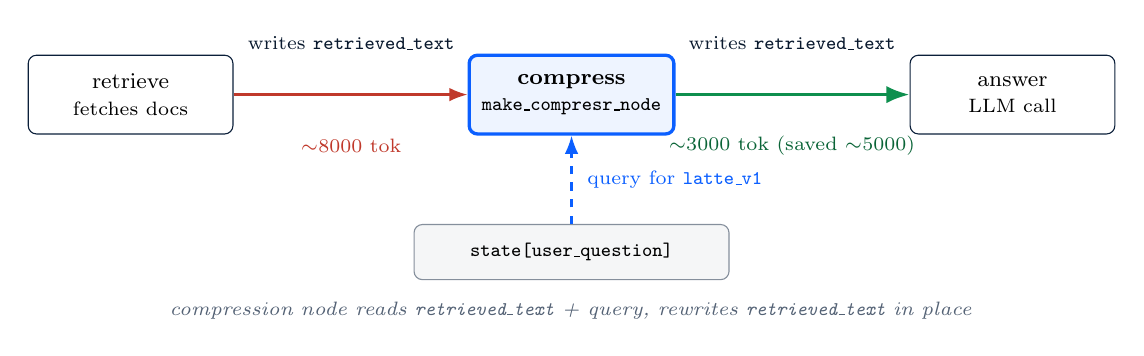
\begin{tikzpicture}[
  font=\footnotesize,
  state/.style={draw=cmpdark!50,rounded corners=3pt,fill=cmpdark!4,
                minimum height=0.7cm,align=center,inner sep=3pt,
                font=\scriptsize\ttfamily},
  n/.style={draw=cmpdark,rounded corners=3pt,fill=white,
            minimum height=1.0cm,minimum width=2.6cm,align=center,inner sep=3pt},
  hl/.style={draw=cmpblue,very thick,fill=boxbg,rounded corners=3pt,
             minimum height=1.0cm,minimum width=2.6cm,align=center,inner sep=3pt,
             font=\footnotesize\bfseries},
  arr/.style={-{Latex},draw=cmpdark!70,thick},
  arrhot/.style={-{Latex},draw=cmpred,thick},
  arrok/.style={-{Latex},draw=cmpgreen,very thick},
]
% Three nodes spread wide
\node[n] (r) at (0,0) {retrieve\\\scriptsize fetches docs};
\node[hl] (c) at (5.6,0) {compress\\\scriptsize \texttt{make\_compresr\_node}};
\node[n] (a) at (11.2,0) {answer\\\scriptsize LLM call};

% State field above each arrow
\node[font=\scriptsize\color{cmpdark!80!black}] at (2.8,0.65) {writes \texttt{retrieved\_text}};
\node[font=\scriptsize\color{cmpdark!80!black}] at (8.4,0.65) {writes \texttt{retrieved\_text}};

% Arrows with token-size annotations BELOW
\draw[arrhot] (r) -- (c);
\node[font=\scriptsize\color{cmpred}] at (2.8,-0.65) {$\sim$8000 tok};

\draw[arrok] (c) -- (a);
\node[font=\scriptsize\color{cmpgreen!70!black}] at (8.4,-0.65) {$\sim$3000 tok (saved $\sim$5000)};

% Query injection from state, shown below
\node[state,minimum width=4.0cm] (q) at (5.6,-2.0) {state[\texttt{user\_question}]};
\draw[->,>=Latex,dashed,cmpblue,thick] (q.north) --
       node[right,font=\scriptsize\color{cmpblue},xshift=2pt]
       {query for \texttt{latte\_v1}} (c.south);

% Caption
\node[font=\scriptsize\itshape\color{cmpdark!70},below=0.15cm of q,text width=11cm,align=center]
   {compression node reads \texttt{retrieved\_text} + query, rewrites \texttt{retrieved\_text} in place};
\end{tikzpicture}
\end{center}

% =====================================================================
\section{Part 2 --- The web search tool}
% =====================================================================

\subsection{Why we need a web search tool at all}

LLMs hallucinate when asked about anything outside training cut-off or anything narrow (specific companies, recent news, niche prices). For analyst-style prompts (``analyse the competitive landscape for X'') there are only two correct outcomes without grounding: refusal (useless) or fabrication (worse). A web search tool fixes that by letting the model fetch live evidence at runtime.

\noindent\textbf{Three jobs the tool performs:} \textbf{(1)} \emph{Recency} --- reach content created after the model's training cut-off; \textbf{(2)} \emph{Verifiability} --- return citable URLs users can audit; \textbf{(3)} \emph{Specificity} --- surface long-tail facts the model never memorised.

\noindent\textbf{Why it matters \emph{specifically} for Compresr.} A search call typically returns 3--10 hits with titles, URLs, and snippets/extracts --- 2--10k tokens per call --- and that text feeds every subsequent turn. This is the single biggest source of token bloat in agent loops, and it is exactly what the SDK exists to remove:

\begin{center}
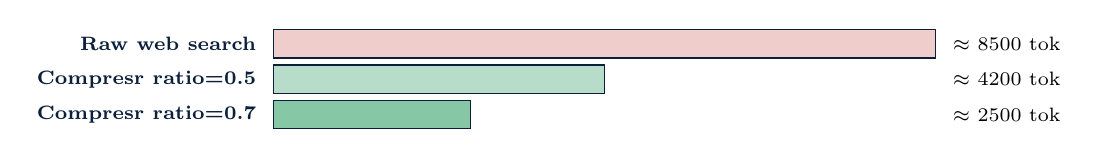
\begin{tikzpicture}[
  font=\scriptsize,
  bar/.style={rectangle,draw=cmpdark,minimum height=0.36cm},
]
\node[anchor=east,font=\scriptsize\bfseries\color{cmpdark}] at (0,0.5) {Raw web search};
\node[bar,minimum width=8.4cm,fill=cmpred!25] at (4.3,0.5) {};
\node[anchor=west] at (8.6,0.5) {$\approx$ 8500 tok};

\node[anchor=east,font=\scriptsize\bfseries\color{cmpdark}] at (0,0.05) {Compresr ratio=0.5};
\node[bar,minimum width=4.2cm,fill=cmpgreen!30] at (2.2,0.05) {};
\node[anchor=west] at (8.6,0.05) {$\approx$ 4200 tok};

\node[anchor=east,font=\scriptsize\bfseries\color{cmpdark}] at (0,-0.4) {Compresr ratio=0.7};
\node[bar,minimum width=2.5cm,fill=cmpgreen!50] at (1.35,-0.4) {};
\node[anchor=west] at (8.6,-0.4) {$\approx$ 2500 tok};
\end{tikzpicture}
\end{center}

\noindent The web search tool and the compression layer are designed to be used \emph{together}.

\subsection{What \texttt{WebSearchTool} actually is}

A thin factory returning a regular LangChain \texttt{BaseTool} backed by either:
\begin{itemize}
  \item \textbf{Tavily} (default) --- via \texttt{langchain\_tavily.TavilySearch}. Supports \texttt{allowed\_domains}/\texttt{blocked\_domains}.
  \item \textbf{Brave} --- via \texttt{langchain\_community.tools.BraveSearch}, wrapped in a \texttt{StructuredTool} with an explicit pydantic \texttt{query} schema (without it, Anthropic tool-use emits an empty args dict because upstream Brave ships with \texttt{args\_schema=None}).
\end{itemize}

\begin{lstlisting}
search = WebSearchTool.tavily(api_key=TAVILY_KEY, max_results=5,
                              allowed_domains=["nytimes.com", "reuters.com"])
# OR
search = WebSearchTool.brave(api_key=BRAVE_KEY, max_results=5)

resp = client.messages.create(
    model="claude-sonnet-4-6", max_tokens=512,
    messages=[{"role": "user", "content": "Analyse competitive landscape for X"}],
    tools=[search],
)
\end{lstlisting}

\subsection{Difference vs.\ Anthropic's \texttt{web\_search\_20250305}}

Anthropic's \href{https://platform.claude.com/docs/en/agents-and-tools/tool-use/web-search-tool}{server-side web search} (\texttt{type: "web\_search\_20250305"}) and the Compresr \texttt{WebSearchTool} look alike --- both let Claude search the web --- but architecturally they are different things. \textbf{Anthropic's is not a chain in your process: it is a black box behind the API.} The model emits a \texttt{server\_tool\_use} block, Anthropic's infrastructure runs the search, and you get back opaque \texttt{web\_search\_tool\_result} blocks with citation URLs --- but the underlying hit content never enters your process in raw form. You cannot intercept it; therefore Compresr cannot compress it. Compresr's tool runs \emph{client-side}, so the result lands in your process as plaintext, and the middleware can read and shrink it.

\begin{center}
\renewcommand{\arraystretch}{1.1}
\footnotesize
\begin{tabular}{@{}p{3.6cm}p{5.5cm}p{5.5cm}@{}}
\toprule
& \textbf{Anthropic \texttt{web\_search\_20250305}} & \textbf{Compresr \texttt{WebSearchTool}}\\
\midrule
Where search runs & Anthropic servers (opaque) & Your process (LangChain tool)\\
Result visibility & Encrypted / not in your process & Plaintext, inspectable\\
Compressible by Compresr & \color{cmpred}\textbf{No} --- nothing to intercept & \color{cmpgreen}\textbf{Yes} --- the design goal\\
Search backends & Anthropic's curated index & Tavily, Brave (pluggable)\\
Billing & Per-search via Anthropic & Direct to Tavily / Brave\\
Domain filtering & Limited & \texttt{allowed/blocked\_domains} (Tavily)\\
Cross-provider & Anthropic only & Same code on Claude / GPT / Gemini\\
Logging / auditing & Not possible & Full visibility in your process\\
\bottomrule
\end{tabular}
\end{center}

\noindent\textbf{Why we forbid the server-side tool.} It is not a chain we can sit in --- it is a sealed call behind the API. Tools and middleware live in your process; the server tool's payload never gets there. With no interception point, there is no compression. Use Tavily or Brave and the middleware can do its job.

\subsection{Migration from \texttt{robust\_client.call\_with\_retry}}

\begin{lstlisting}
# BEFORE -- server-side tool, opaque to your code
tools=[{"type": "web_search_20250305", "name": "web_search",
        "max_uses": WEB_SEARCH_MAX_USES}]

# AFTER -- client-side, compressible
from compresr import WebSearchTool
tools=[WebSearchTool.brave(api_key=BRAVE_KEY, max_results=3)]
# or: WebSearchTool.tavily(api_key=TAVILY_KEY, max_results=3)
\end{lstlisting}

\noindent The wrapping \texttt{RobustClient} is unchanged. It still calls \texttt{self.client.messages.create(**request\_params)}; what changed is that \texttt{self.client} is now \texttt{CompressionClient} and the tool produces compressible plaintext instead of opaque server-tool output.

\subsection{Getting the final result --- three surfaces, same engine}

Compresr exposes three equivalent surfaces on the same client. Pick by ergonomics; behaviour and middleware path are identical. The model lives at the \emph{call site}, just like Anthropic's and OpenAI's own SDKs.

\noindent\textbf{1.\ Anthropic shape} --- response is an \texttt{anthropic.types.Message}; iterate \texttt{response.content} for text and \texttt{tool\_use} blocks (matches the existing \texttt{RobustClient} code path):

\begin{lstlisting}
resp = client.messages.create(
    model="claude-sonnet-4-6", max_tokens=512,
    messages=[{"role": "user", "content": "Analyse competitor landscape for X"}],
    tools=[WebSearchTool.brave(api_key=BRAVE_KEY, max_results=3)],
)
text = "".join(b.text for b in resp.content if hasattr(b, "text"))
stop = resp.stop_reason          # "end_turn" / "tool_use" / "max_tokens"
usage = resp.usage               # input_tokens, output_tokens, ...
\end{lstlisting}

\noindent\textbf{2.\ OpenAI shape} --- response is the OpenAI \texttt{ChatCompletion}; read \texttt{choices[0].message.content}:

\begin{lstlisting}
client_oai = CompressionClient(
    api_key=COMPRESR_KEY,
    llm="openai", llm_api_key=OPENAI_KEY,
    compression={"target_compression_ratio": 0.5},
)
resp = client_oai.chat.completions.create(
    model="gpt-4o-mini",
    messages=[{"role": "user", "content": "Analyse competitor landscape for X"}],
    tools=[WebSearchTool.tavily(api_key=TAVILY_KEY, max_results=5)],
)
text = resp.choices[0].message.content
finish = resp.choices[0].finish_reason
\end{lstlisting}

\noindent\textbf{3.\ Native \texttt{client.run(...)}} --- provider-agnostic. Returns a \texttt{NormalizedResult} with the same fields no matter which provider you target. Best for code that should work across Claude / GPT / Gemini:

\begin{lstlisting}
result = client.run(
    prompt="Analyse competitor landscape for X",
    model="claude-sonnet-4-6",   # or "gpt-4o-mini" / "gemini-1.5-pro" with right llm=
    tools=[WebSearchTool.brave(api_key=BRAVE_KEY, max_results=3)],
    max_tokens=512, temperature=0.2,
)
result.text          # str  -- final assistant text
result.tool_uses     # list -- [{id, name, input}, ...]
result.citations     # list -- [Citation(url, title, cited_text), ...] normalised
result.stop_reason   # str  -- "end_turn" / "tool_use" / ...
result.usage         # dict -- {input_tokens, output_tokens, ...}
result.raw           # the underlying provider message (escape hatch)
\end{lstlisting}

\noindent\textbf{Per-call LLM knobs.} \texttt{temperature}, \texttt{top\_p}, \texttt{stop\_sequences}, \texttt{seed}, \texttt{presence\_penalty}, etc.\ pass through to the underlying chat model via \texttt{.bind(...)} on each call --- the cached model is never mutated, so switching knobs between calls is safe.

\end{document}
